\chapter{統計を用いた画像再構成手法の改善}
\newpage
\section{概要}
本章では, 骨のような下肢組織の断層画像取得の際の精度の向上のための統計的処理の検討を述べる.
\section{下肢組織の構造}
下肢組織は, 大きく分けて上腿と下腿の2つに分けられる(\figref{kashisoshiki}). 上腿には大腿骨が, 下腿には脛骨および腓骨がある. 将来的に診断装置として本研究を活用する際には, 上腿あるいは下腿にせん断波を与えた際の筋組織などの挙動を観察し, その健康状態を評価することを想定しているが, 現段階では上腿あるいは下腿のどちらがより顕著にせん断波に対する機械的特性を反映させるかわかっていない. また, 上腿は骨が大腿骨1本のみであるため, 画像処理はより単純になるが, 将来的な診断装置としての発展を考えると, 下腿のように衣服を少しあげるだけで診断ができるというのは大きな魅力になる. そこで, 本章では上腿および下腿の両方においてシミレーションを行うことにする. 
\\\ \ 下肢組織の大腿骨, 脛骨, 腓骨などのような骨が超音波CTで断層画像を取得した時のノイズの原因になる可能性がある. そこで, 本研究では, ノイズを軽減する画像再構成手法および画像処理を考案する. 
\begin{figure}[H]
  \begin{center}
    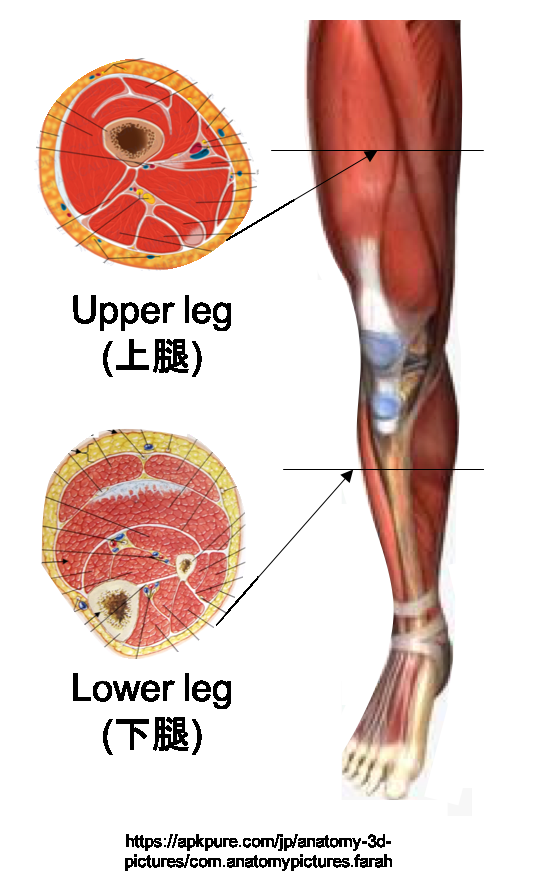
\includegraphics[width=50mm]{fig/kashisoshiki.pdf}
  \end{center}
  \caption{下肢組織の構造}
  \figlab{kashisoshiki}
\end{figure}
\section{シミュレーション系の設定}
本研究は下肢組織を対象としているために\figref{daitai}, \figref{keikotsu},  \figref{hikotsu}に示すような3種のシミュレーション系を設定した. 計算領域は, 110mm$\times$110mmであり, グリッドサイズは0.21mm$\times$0.21mmである. また, 周波数は1.6MHz, 筋肉および皮下組織内の音速は1500m/s, 大腿骨, 脛骨および腓骨の音速は2700m/sとした(表\ref{simulation_settei}). 水中の音速は1500m/sであるが, まずはシミュレーションの条件を単純化するべく, 筋肉および皮下組織内の音速も1500m/sで近似している. そのため, 今回のシミュレーションでは水の中に骨のみがあるようなモデルでシミュレーションを行なった. \figref{daitai}, \figref{keikotsu},  \figref{hikotsu}を取り囲むように, 直径100mm, 圧電素子数1024のリング型アレイトランスデューサが設置されている. 
\begin{figure}[H]
 \begin{minipage}{0.325\hsize}
  \begin{center}
   \includegraphics[width=40mm]{fig/daitai.pdf}
  \end{center}
  \caption{大腿骨モデル}
   \figlab{daitai}
 \end{minipage}
 \begin{minipage}{0.325\hsize}
 \begin{center}
  \includegraphics[width=40mm]{fig/keikotsu.pdf}
 \end{center}
  \caption{脛骨モデル}
  \figlab{keikotsu}
 \end{minipage}
 \begin{minipage}{0.325\hsize}
 \begin{center}
  \includegraphics[width=40mm]{fig/hikotsu.pdf}
 \end{center}
  \caption{脛骨・腓骨モデル}
  \figlab{hikotsu}
 \end{minipage}
\end{figure}
\begin{table}[H]
\centering
\caption{シミュレーション系の設定}
\label{simulation_settei}
\begin{tabular}{|c|c|c|}
\hline
組織 & 直径[mm] & 計測周波数$f$[Hz]  \\ \hline
筋肉 & - &      1500 \\ \hline
皮下組織   & - &      1500\\ \hline
大腿骨  & 30 &     2700 \\ \hline
脛骨 & 30 &     2700 \\ \hline
腓骨  & 7 &     2700  \\ \hline
\end{tabular}
\end{table}
